\documentclass{scrreprt}
\usepackage{etex}
\usepackage[ngerman]{babel}
\usepackage[utf8]{inputenc}
\usepackage[T1]{fontenc}
\usepackage{amsmath, amssymb}
\usepackage{graphicx}

\usepackage{pgfplots}
\pgfplotsset{compat=1.11}
\usepgfplotslibrary{external}
\usepackage{pgfplotstable}

\usepackage{booktabs}
\usepackage{multirow}
\usepackage{longtable}
%\usepackage{ulsy}
%\usepackage{pst-all}
\usepackage{picture}
\usepackage[automark]{scrpage2}
\usepackage{caption}
\pagestyle{scrheadings}
\ihead[]{Friedrich Hübner 2897111}
\ohead[]{Fiona Paulus 2909625} 


\author{Friedrich Hübner 2897111\\
	Fiona Paulus 2909625}
\title{Computerphysik\\Hausarbeit 6}

\begin{document}
	\maketitle
	\newpage
	
\chapter*{Aufgabe 1: Gammalinie}
\section*{allgemeine Hinweise}
Das Programm zu Aufgaben b) und c) wurde unter Linux-Mint mit 'g++ -std=c++11 -g -Wall -Wextra b.cpp -o b.exe' kompiliert.\\
Das Programm zu d) wurde unter Windows mit 'g++ -o abgabe6\_fit.exe -Wall -Wextra -std=c++0x -O2 -static abgabe6\_fit.cpp' kompiliert.
\section*{a)}
Das Plotten der Datei "profile.dat" ergibt das Spektrum eines Gammastrahlers. Es wird die Impulsrate gegen die Energie aufgetragen.
\begin{center}
	\includegraphics*[scale=0.7]{a.jpeg}
	\captionof*{figure}{Spektrum eines Gammastrahlers}
\end{center}

\section*{b}
Aus dem Spektrum des Gammastrahlers aus a) soll der Kosmische Mikrowellen Hintergrund berechnet werden. Dazu wird eine Spline-Interpolation verwendet, welche mithilfe von festglegten Stützstellen $x_i$ und den dazugehörigen Stützwerten $y_i$ ein Polynom 3.Grades an die Messdaten fittet ("b.cpp").

Dieses Polynom und seine Ableitungen werden für jedes Intervall berechnet.

\[S_i(x)=a_i(x-x_i)^3+b_i(x-x_i)^2+c_i(x-x_i)+d_i\]
\[S'_i(x)=3a_i(x-x_i)^2+2b_i(x-x_i)+c_i\]
\[S''_i(x)=6a_i(x-x_i)+2b_i\]

\[0 \leq i \leq n\]
n: Anzahl der Stützstellen

Um das Gleichungssystem zu lösen werden Bedingungen aufgestellt.
Die Gesamtfunktion muss stetig sein, somit müssen die Polynome der Intervalle an den Stützstellen übereinstimmen.

\[S_i(x_i)=S_{i-1}(x_i)\]
\[S'_i(x_i)=S'_{i-1}(x_i)\]
\[S''_i(x_i)=S''_{i-1}(x_i)\]
Außerdem müssen die Funktionswerte an den Stützstellen mit den zugehörigen Stützwerten übereinstimmen.

\[S_i(x_i)=y_i\]
\[S_{n-1}(x_n)=y_n\]
Und die Krümmung an den Rändern der Gesamtfunktion soll verschwinden.

Die Interpolation wird mit folgenden Stützwerten und dazugehörigen Stützstellen durchgeführt:

\begin{center}
		\begin{tabular}{cccc}
			Stützwert i & Messwert k & Stützstelle $x_i$ & Stützwert $y_i$\\
			\\
			0 & 15 & 50 & 887.992\\
			1 & 415 & 250 & 701.793\\
			2 & 715 & 400 & 623.281\\
			3 & 1015 & 550 & 486.757\\
			4 & 1415 & 750 & 266.316\\
			5 & 1715 & 900 & 209.190\\
		\end{tabular}
\end{center}

Daraus werden die Abstände $h_i=x_{x+1}-x_i$ $0 \leq i \leq 4$ zwischen den Stützpunken berechnet, mit deren Hilfe die Koeffizienten A,B,C,D berechnet werden.

\[A_i = h_{i-1}\]
\[B_i = 2(h{i-1}+h_i)\]
\[C_i = h_i\]
\[D_i = g(\frac{y_{x+1}-y_i}{h_i}-\frac{y_i-y_{i-1}}{h_{i-1}})\]
Daraus werden weitere Koeffizienten berechnet:


\[B'_i = B_i-C_{i-1}\frac{A_i}{B_{i-1}}\]
\[D'_i = D_i-D_{i-1}\frac{A_i}{B_{i-1}}\]
mit $B_1=B'_1$ und $D_1=D'_1$
Außerdem gilt:
\[X_i=y''_i\]
\[X_4 = \frac{D'_4}{B'_4}\]
wodurch sich alle weiteren $X_i$ rekursiv berechnen lassen.

Aus diesen Koeffizienten ergeben sich nun die Koeffizienten der Polynome a,b,c und d.

\[a_i = \frac{y''_{i+1}-y''_i}{6h_i}\]
\[b_i = \frac{y''_i}{2}\]
\[c_i = \frac{y_{i+1}-y_i}{h_i}-\frac{h_i(y''_{i+1}+2y''_i)}{g}\]
\[d_i = y_i\]

Mit diesen Koeffizienten ergeben sich die Polynome mit denen die Funktion des Kosmischen Hintergrunds beschrieben wird.

\begin{center}
	\includegraphics*[scale=0.7]{b.jpeg}
	\captionof*{figure}{Spektrum eines Gammastrahlers und Kosmischer Mikrowellenhintergrund}
\end{center}
\section*{c)}
Nun wird die Funktion des Kosmischen Hintergrunds von der Gammalinie subtrahiert um die reine Strahlung des Gammastrahlers zu erhalten.("b.cpp")

\begin{center}
	\includegraphics*[scale=0.7]{c.jpeg}
	\captionof*{figure}{Spektrum eines Gammastrahlers ohne kosmischen Mikrowellenhintergrund}
\end{center}

\section*{d)}
An die bereinigten Daten soll jetzt eine Gaussfunktion gefittet werden. Dazu wird das Gauss-Seidel-Verfahren mit dem Levenberg-Marquard-Verfahren verwendet.

\subsection*{Gauss-Seidel}
Das Gauss-Seidel-Verfahren wird wie in der Vorlesung besprochen implementiert (siehe Vorlesung für Details). In jedem Schritt werden die Parameter $a$ angepasst. Dazu berechnet man mit den aktuellen Parametern die Matrix $A$ und den Vektor $b$ (im Skript $\beta$).
Das Inverse von b unter dieser Matrix ist gerade der Schritt $\Delta a$, um den man $a$ verschiebt. Danach beginnt der Prozess von vorne, solange bis der maximale relative Fehler $\max\limits_i \frac{\Delta a[i]}{a[i]} < \epsilon = 10^{-5}$. Allerdings wird das Programm künstlich nach 100000 Iterationen abgebrochen um mögliche Endlosschleifen zu verhindern.\\

Um $A$ und $b$ zu berechnen, benötigt man die Funktion und die partiellen Ableitungen nach den Parametern.\\
\begin{align*}
f(x) &= Ne^{-\frac{(x-\mu)^2}{2\sigma^2}}\\
\frac{\partial f}{\partial \mu} &= \frac{x-\mu}{\sigma^2} Ne^{-\frac{(x-\mu)^2}{2\sigma^2}}\\
\frac{\partial f}{\partial \sigma} &= \frac{(x-\mu)^2}{\sigma^3} Ne^{-\frac{(x-\mu)^2}{2\sigma^2}}\\
\frac{\partial f}{\partial N} &= e^{-\frac{(x-\mu)^2}{2\sigma^2}}\\
\end{align*}
Die Indizes der Parameter wurde wie folgt festgelegt:\\
\begin{center}
\begin{tabular}{ccc}
\toprule
Index & Parameter & Startwert\\
\midrule
0 & $\mu$ & 650\\
1 & $\sigma$ & 50\\
2 & $N$ & 4000\\
\bottomrule
\end{tabular}
\end{center}

\subsection*{Levenberg-Marquard}
Auch hier hält sich die Implementierung an die Vorlesung. Man startet mit einem $\lambda = 0.0003$. Vor jeder Iteration verkleinert man $\lambda$ mit dem Faktor $\gamma = \frac{1}{5}$.
Hat man $A$ und $b$ berechnet, dann invertiert man nicht $A$, sondern $A + \lambda\cdot\mathbb{I}$. Nach der Invertierung vergleicht man die Änderung von $\chi^2$. Wurde $\chi^2$ kleiner, dann fährt wie gewohnt fort, sonst erhöht man $\lambda$ solange mit dem Faktor $\delta = 5$, bis das neue $\chi^2$ kleiner als das alte ist (siehe Vorlesung für Details).\\

Sollte es nicht gelingen eine Matrix zu invertieren, so wird $\lambda$ um den kleinen Faktor $1.00001$ erhöht, um eine geringfügig andere Matrix zu erhalten, die dann hoffentlich invertierbar ist.\\

Weiterhin bricht das Programm ab, sollte $\lambda$ größer als $10^{200}$ werden.

\subsection*{Matrix invertieren: LU-Zerlegung}
Für den Algorithmus muss man Matrizen invertieren können. Dies geschieht über eine LU-Zerlegung wie in der Vorlesung besprochen. Kann eine Matrix nicht LU-Zerlegt werden, weil ein Diagonalelement von $U$ 0 ist, so wird in die Matrix oben links der Wert $nan$ geschrieben oder eine leere Matrix/Vektor zurückgegeben (siehe Implementierung). Dadurch kann man während des Programmes erkennen, dass die Matrix nicht invertiert werden konnte.

\subsection*{Fehler}

Die Fehler der Parameter werden wie in der Vorlesung über das Inverse der Normalenmatrix bestimmt. Dazu wird der Term zweiter Ordnung in den partiellen Ableitungen vernachlässigt (weil der Faktor davor sehr klein ist). Die Standartabweichungen sind dann die Wurzeln der Diagonalelemente der Inversen der Normalenmatrix.

\subsection*{Ergebnis}
Das Programm liefert folgende Werte:\\

\begin{center}
\begin{tabular}{ccc}
\toprule
Index & Parameter & Wert\\
\midrule
0 & $\mu$ & $657.01873 \pm 0.00077$\\
1 & $\sigma$ & $19.12992 \pm 0.00077$\\
2 & $N$ & $4251.8642 \pm 0.1487$\\
\bottomrule
\end{tabular}
\end{center}

\begin{center}
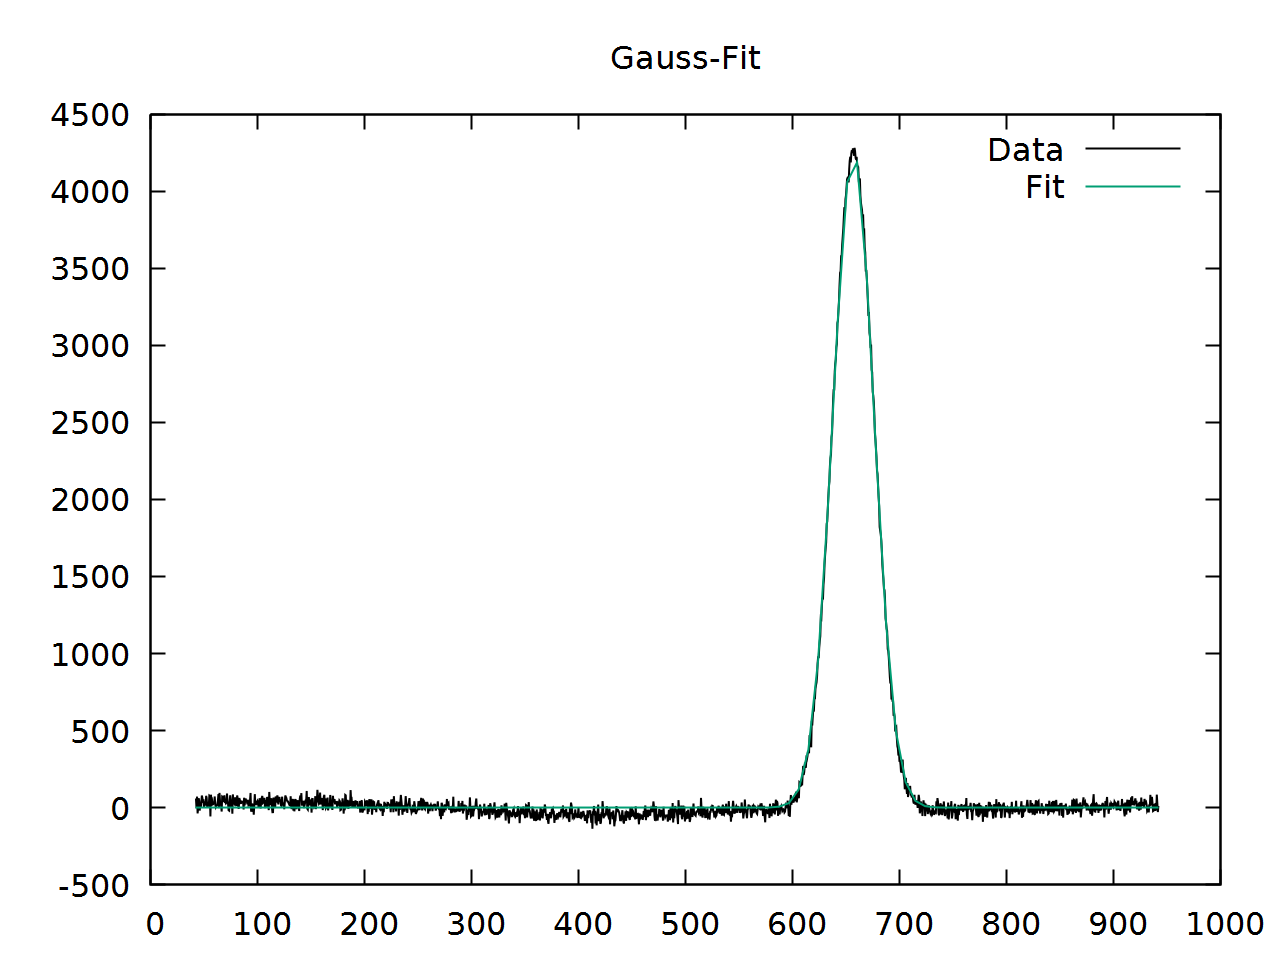
\includegraphics[scale=0.3]{d/plot_fit.png}
\captionof{figure}{Fit mit Daten}
\end{center}

\section*{e)}
Das Integral über eine Gausskurve lautet:\\

\begin{align*}
\int\limits_{-\infty}^{\infty} Ne^{-\frac{(x-\mu)^2}{2\sigma^2}} dx = \sqrt{2\pi}\sigma\cdot N
\end{align*}

Die Anzahl der Gesamtimpulse lautet also: $\sqrt{2\pi}\cdot 19.12992\cdot 4251.8642 = 203883.68$

\section*{sonstige abgegebene Datein}
\subsection*{plot.plt}
Plotdateien für Aufgabenteile a),b) und c)
\subsection*{cmb.dat}
Ausgabedatei des Programms "b.cpp" für den Aufgabenteil b)
\subsection*{profile\_cmb.dat}
Ausgabedatei des Programms "b.cpp" für den Aufgabenteil c)
\subsection*{plot\_fit.plt}
Plotdatei für Aufgabe d)
\end{document}